\documentclass[a4paper,12pt]{extarticle}

% geometry
\usepackage[top=25mm, bottom=25mm, left=25mm, right=20mm]{geometry}
\renewcommand{\baselinestretch}{1.5}

% language
\usepackage[croatian]{babel}
\usepackage[utf8]{inputenc}

% images
\usepackage{graphicx}
\usepackage{float}

% numbering
\renewcommand{\thesection}{\arabic{section}.}
\renewcommand{\thesubsection}{\thesection\arabic{subsection}.}
\renewcommand\thefigure{\thesection\arabic{figure}}
\renewcommand{\theequation}{\arabic{section}--\arabic{equation}}

% additional
\usepackage{titlesec}
\usepackage{amsmath}
\newcommand{\sectionbreak}{\clearpage}
\usepackage{times}
\setlength{\parindent}{1.5em}
\setlength{\parskip}{0.8em}
	
\begin{document}


\begin{titlepage}
	\centering
	{\bfseries SVEUČILIŠTE JOSIPA JURJA STROSSMAYERA U OSIJEKU\par}
	{\bfseries FAKULTET ELEKTROTEHNIKE, RAČUNARSTVA I INFORMACIJSKIH TEHNOLOGIJA\par}
	
	\vspace{2cm}
	{\bfseries Sveučilišni studij\par}

	\vspace{4cm}
	{\huge\bfseries NEFOTOREALISTIČNI PRIKAZ 3D MODELA KORIŠTENJEM CEL-SHADERA\par}
	
	\vspace{1cm}
	{\bfseries Diplomski rad\par}
	
	\vspace{2cm}
	{\Large Stjepan Udovičić\par}
	
	\vfill
	{Osijek, 2016.\par}
\end{titlepage}

\tableofcontents




% TODO:
% 1. Kako navesti izvor modela
% 2. Trebam li pisati da su slike/grafovi moji?

\section{Uvod}

Razvojem novih tehnologija i uređaja, postoji kontinuirana potreba za napretkom računalne grafike, kako u mogućnostima tako i performansama. Iako je primarni fokus ovoga napretka bio foto realističan prikaz, ponekada je potreban drugačiji pristup iz praktičnih ili estetskih razloga. Kako bi grafička sučelja omogućila slobodu obrade slike, a u isto vrijeme i kontrolu nad performansama, koriste se programska sučelja - API \footnote{engl. Application programming interface - set definicija, protokola i alata za izradu programa}. Jedno od najpoznatijih grafičkih aplikacijski sučelja je OpenGL \footnote{engl. Open Graphics Library}.

Za prikaz 3D modela u realnom vremenu, potrebno je izvršiti niz zahtjevnih matematičkih operacija kako bi se odredio položaj i boja svake točke \footnote{engl. pixel - najmanja jedinica u računalnoj slici} na ekranu. Takve operacije najčešće nisu dovoljno brze na procesoru samog računala, pa se za te potrebe koristi specijalizirano sklopovlje grafičkih kartica. Pristup tom sklopovlju omogućen nam je preko OpenGL-a koji omogućava izvršavanje vlastitih programa izravno na grafičkim karticama, pri čemu se ostvaruje velika brzina rada zbog paralelnog načina obrade podataka.

U ovom radu opisano je kako se koristi moderni OpenGL za prikaz modela. Opisuje se način učitavanja podataka i njihov prijenos u memoriju grafičke kartice. Izradom vlastitih programa za sjenčanje \footnote{engl. shader}, prikazano je kako se vrši programiranje grafičkih kartica za obradu slike s ciljem postizanja specijalnih efekata.

\subsection{Zadatak diplomskog rada}

Cilj je razviti prilagođeni sustav sjenčanja za OpenGL koji će 3D modele prikazivati nefotorealistično u svrhu stvaranja dojma kako su ručno nacrtani. Potrebno je razviti aplikaciju koja omogućava učitavanje  3D modela iz datoteke te ga prikazuje korištenjem prilagođenog sustava sjenčanja. Funkcionalnost razvijene aplikacije treba testirati prikazivanjem nekoliko 3D modela.

\section{OpenGL aplikacijsko sučelje}

OpenGL razvio se kao nasljednik IrisGL-a \footnote{engl. Integrated Raster Imaging System Graphics Library}. Njegov glavni nedostatak bio je što su mogućnosti samog sučelja ovisile o mogućnostima sklopovlja, te se nije mogao primijeniti na različitim uređajima. Zbog potrebe za izradom standarda, početkom 1990-ih godina tvrtka Silicon Graphics Inc. (SCI) započela je sa izradom OpenGL specifikacije kako bi formalno definirala aplikacijsko programsko sučelje (API) prema grafičkim karticama. Godine 1992., prva verzija OpenGl-a je objavljena. Od 2016.g. ne-profitna grupa Khronos zadužena je za razvoj OpenGL-a \cite{opengl-wiki-hostory}.

Primarni zadatak ovog API-a je prikaz 2D i 3D vektorske grafike. On omogućuje komunikaciju sa grafičkim procesorom (GPU) s ciljem sklopovskog ubrzanja grafičkog prikaza, neovisno o programskom jeziku i operativnom sustavu.

Zbog svoje proširenosti i upotrebe, postao je industrijski standard. Podržan je na velikom broju uređaja, od računala do pametnih telefona. Ima široku primjenu u industriji (CAD \footnote{engl. Computer-Aided Design}, GIS \footnote{engl. Geographic Information System}, simulacijama i vizualizacijama) te u izradi računalnih igara.

\subsection{OpenGL grafički cjevovod}

U svojim početcima, prilikom rada s računalnom grafikom nije bilo puno mjesta za manipulaciju sa slikom. Grafičko sklopovlje nije omogućavalo puno manipulacije sa bojom i pozicijom objekata na ekranu. Računalo je \emph{slalo} opise vektore i teksturu koju oni stvaraju, dok su grafičke kartice bila zadužene za stvaranje slike iz ta dva dobivena podatka.

Takav način rada podrazumijevao je da se sva potreban kalkulacija (tranformacija koordinata - pomak) i sjenčanje prethodno odrade na samom računalu, prije nego što se pošalju grafičkoj kartici za prikaz. Glavni nedostatak tog pristupa je što svu kalkulaciju morala obrađivati centralna procesorska jedinica (CPU) koja osim što nije bila dizajnirana za takve operacije, je morala obrađivati i niz drugih podataka istovremeno.

Iz tog razloga, pojavila se potreba za programabilnim \emph{grafičkim cjevovodom} \footnote{engl. Graphival pipline} koji bi omogućio manipulaciju podacima na grafičkoj kartici. OpenGL cjevovod sastoji se od 7. komponenti\cite{opengl-wiki-pipeline}, prikazanih na slici \ref{fig:pipeline}.

\begin{figure}[H]
\centering\fbox{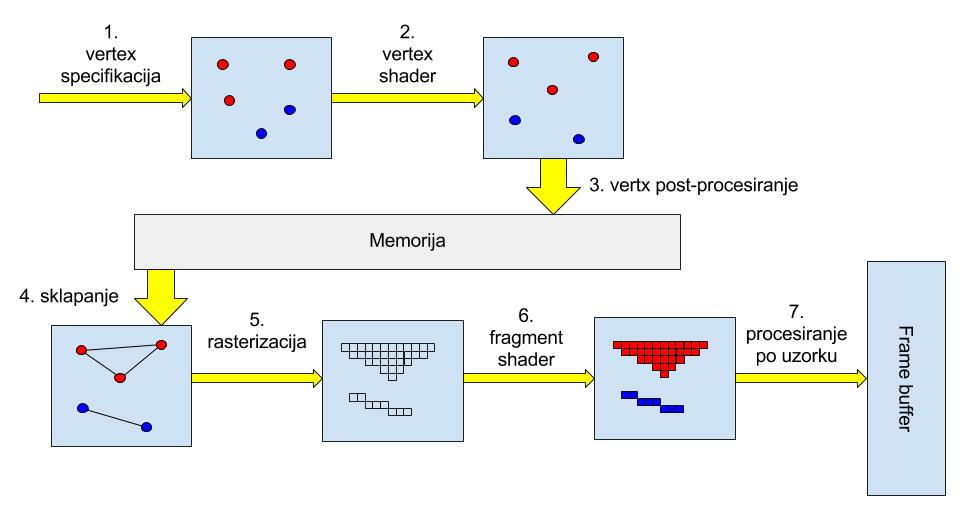
\includegraphics[scale=0.4]{pipeline.jpg}}
\caption{Dijagram toka OpenGL cjevovoda}
\label{fig:pipeline}
\end{figure}

\begin{enumerate}
\item \textbf{Vertex specifikacija:} U ovom koraku aplikacija prenosi podatke grafičkoj kartici - opise vertex-a \footnote{Točka u trodimenzionalnom prostoru. Osim pozicije, vertex može sadržavati i druge informacije, poput boje}. Način na koji će se vertex tumačiti/iscrtavati se kasnije obrađuje.

\item \textbf{Vertex shader:} Izvršavanje vertex shader korisničkog programa. Cilj ovog koraka je transformirati ulaznu poziciju vektora u njegov krajnji oblik. Ovdje se najčešće vrše transformacije s ciljem postizanja pogleda iz perspektive, rotacije i uvećanja. U ovoj fazi pokreće se i geometrijski shader, koji radi kao i vertex shader, samo na razini ploha.

\item \textbf{Vertx post-procesiranje:} Rezultati prošlog koraka spremaju se za na to predviđene memorijske lokacije.

\item \textbf{Sklapanje ploha:} U ovome koraku, grafički procesor sklapa ploha od unaprijed obrađenih vertexa.

\item \textbf{Rasterizacija:} Sklopljene plohe razdvajaju se na fragment koji se prosljeđuju dalje kako bi im se odredila boja, odnosno tekstura.

\item \textbf{Fragment shader:} Svaki fragment se prosljeđuje korisničkom programu fragment shaderu) čiji izlaz predstavlja boju danoga fragmenta.

\item \textbf{Procesiranje po uzorku:} Ovaj korak služi za izvršavanje raznih testova koji mogu utjecati na krajnji rezultat, primjerice test dubine (ukoliko se fragment nalazi iza nekog drugog, vjerojatno neće biti prikazan). Također ovdje se vrše operacije i odbacivanja fragmenata koji nisu na vidljivom djelu ekrana, stapanje boja i sl.

\end{enumerate}

Kod ovoga koraka bitno je napomenuti kako su procesi optimizirani na način da se što više operacija može izvršavati paralelno. Današnje grafičke kartice imaju i po nekoliko stotina jezgri koje mogu paralelno raditi, što omogućava paralelno izvršavanje nekoliko shadera istovremeno, što u konačnici rezultira velikom brzinom obrade podataka, nešto što nije moguće na centralnoj procesorskoj jedinici,

\subsection{Shaderi i GLSL}

Kao što je opisano u prethodnom poglavlju, shaderi su najbitnije komponente progamabilnog grafičkog cjevovoda. Oni su zapravo male korisničke aplikacije koje se izvode paralelno, i obrađuju manji set informacija od jednom.

Korisničke aplikacije za vertex i fragment shader (opcinoalno i geometrijski) se dostavljaju grafičkoj kartici, i zatim komapjliraju u jedan \emph{program} koji se izvodi u sklopu cjevovoda. Bitno je napomenuti da je moguće prirediti više od jednog programa, te ih mijenjati tokom izvođenja.

Shaderi se pišu programskom jeziku koji je posebno dizajniran za ovu primjenu - GLSL \footnote{engl. OpenGL Shading Language}. GLSL programski jezik baziran je na C programskom jezu, i dio je OpenGL specifikacije. Razlikuje se od C-a u nekoliko ključnih stvari: nadograđen je da podržava matrične operacije i tipove podataka. Za razliku od C-a, ne podržava preopterećenje funkcija na osnovu ulaznih parametara niti rekurzivne funkcije.

Svaki shader rasolaže sa nekoliko ulaznih varijabli:

\begin{itemize}

\item \textbf{Ulazne varijable:} Svaki shader imaju svoju glavnu ulaznu varijablu. Za vertex shader to je \emph{position}, vektor s četiri vrijednosti koji opisuje početnu poziciju objekta u 3D prostoru. Četvrta vrijednost (w) označava orijentaciju. U slučaju fragment shadera, stvar je malo složenija, jer se samom fragmentu ne mora nužno dodijeliti samo boja, već se može dodjeliti i komad teksture. Naziv samih varijabli ovisi o načinu učitavanja modela, odnosno ime se proizvoljno dodijeljuje kod učitavanja modela.

\item \textbf{Uniform varijable:} Ovo su varijable koje su dostupne svim shaderima. Njihovu vrijednost postavlja glavni program prije početka rendering procesa, te ona ostaje ista tokom cijelog izvođenja. Ove varijable se najčešće koriste za prijenos MVP\footnote{engl. Model View Projection} matrica, koje su obrađene u sljedećem poglavlju.

\item \textbf{Varying varijable:} Ovo su varijable koje su dostupne svim shaderima, no njihovu vrijednost postavlja jedan shader, kako bi određenu informaciju mogao proslijediti dalje niz cjevovod. Primjerice, normala vertexa ulazni je parametar vertex shadera. No ta vrijednost često je potrbna fragmen shaderu kako bi pravilno odredio sjenčanje objekta. Iz toga razloga, često se definira \emph{varying} varijabla, čija se vrijednost postavlja unutar vertex shadera za daljnje korištenje.
\end{itemize}

Izlaz iz vertex shader-a je varijabla \emph{gl\_Position} \footnote{Interna OpenGL varijabla koja opisuje položaj trenutnog vertexa u 3D prostoru}, dok je izlaz fragment shader-a varijabla \emph{gl\_FragColor} \footnote{Interna OpenGL varijabla koja opisuje boju treutnog fragmenta}. Iako su ovi izlazi nužni za rad, pojedini shaderi su često zaduženi za kalkulaciju i niz drugih \emph{varying} varijabli koje će se koristiti dalje u grafičkom cjevovodu.

\subsection{Transformacije objekta}

Kako je ranije spomenuto, ideja programabilnog grafičkog cjevovoda je pomaknuti grafičke kalkulacije sa centralnog procesora na grafički procesor. To prvenstveno znači rekalkulaciju pozicije i oblika objekta uslijed pomaka samog objekta ili kamere. To se najčešće vrši množenjem kordinata pojedine točke objekta sa takozvanom MVP \footnote{engl. Model View Projection} matricom. MVP matrica se sastoji iz tri dijela \cite{opengl-es-mvp}:

\begin{enumerate}
\item \textbf{Matrica modela:} Matrica koja opisuje osnovne transformacije modela: translaciju, rotaciju i skaliranje. Dobiva se množenjem istoimenih matrica.

\item \textbf{Matrica scene (view):} Budući da se u računalnoj grafici kamera ne pomiče, već se pomiče svijet oko nje - ova matrica služi kako bi ispravno pozicionirala objekt u odnosu na kameru.

\item \textbf{Projekcijska matrica:} Služi za definiranje transformacije s ciljem postizanja željene projekcije. To je najčešće perspektivna projekcija, no može biti ortogonalna i bilo kako drugo definirana.
\end{enumerate}

Sam izračun MVP matrice, obično se vršri na centralnoj procesorskoj jedinici i kao takav se dostavlja grafičkoj kartici. Ona je zatim zadužena da svaki pojedini vertex pozicionira na pravo mjesto, uzimajući MVP matricu u obzir - pomnoži koordinate vertxa sa MVP matricom da dobije konačnu poziciju u prostoru.

Na ovaj način, smanjuje se količina posla koju obavlja centralna procesorska jedinica. Ona samo računa način tranformacije, dok se stvarni pomak modela odvija na samoj grafičkoj kartici, koja je u mogućnosti to obaviti neusporedivo brže, za svaki vertex posebno.

\subsection{WebGL}

WebGL \footnote{engl. Web Graphics Library} je JavaScript grafički API koji je nastao na temelju OpenGL ES 2.0 standarda, te služi za hardwersko ubrzanje prilikom prikazivanja 3D grafike na internet preglednicima. Razvoj standarda vrši Khronos WebGL grupa, a sam standard podržan je od strane svi vodećih internet preglednika koji podržavaju HTML 5 canvas element.

Iako se zapravo ne radi o istom standardu kao i OpenGL, WebGL zadržava što je moguće više sličnosti sa OpenGL-om radi lakog prijenosa aplikacija s jednog API-a na drugi.

Kao i OpenGL, WebGL također ima programabilan grafički cjevovod, uz ograničenje da ne podržava geometrijski shader. Ostatak funkcionalnosti je isti, i ponaša se na identičan način.

\subsection{Modeli u Three.js JSON formatu}

Kao i OpenGL, WebGL propisuje funkcije za pristupanje grafičkom sučelju na vrlo niskoj razini, što za korisnika znači da mora sam voditi računa o alokaciji memorije i prijenosu podataka. Iz tog razloga, postoji mnogo frameworka koji se zaduženi za olakšavanje rada s nekim bazičnim stvarima.

Za potrebe ovoga rada, korišten je three.js \footnote{http://threejs.org/ verzija 73}, WebGL framework koji olakšava poslove poput prijenosa modela u memoriju grafičke kartice, kao i postupak kompajliranja korisničkih sahadera.

Kao format spremanja 3D modela, korišten je three.js JSON format, budući da je s JSON formatom najlakše raditi u \emph{JavaScript}-u. Unutar datoteke, model je opisan kroz nekoliko ključnih elemenata \cite{threejs-json}:

\begin{itemize}
\item \textbf{vertices:} Popis vertex, pri čemu je svaki opisan sa tri koordinate: x,y i z. Ovo polje more biti proizvoljne duljina, ali je bitno da je višekratnik broja 3.

\item \textbf{normals:} Kao i vertex-i, normalne s opisane sa tri koordinate. Njihov broj pak ovisi o vrsti ravnina koju vertex-i opsiuju: trokuti, četverokuti, ...

\item \textbf{faces:} Ovo polje opisuje koji vertexi i normale (opcinalno i teksture i boje) čine jednu plohu. Prvi broj u nizu definira masku pod kojom se učitavaju ostali podaci. Evo nekoliko primjera:

\begin{itemize}

\item \textbf{0, 0,1,2} : Vodeća 0 označava da slijede tri vertexa koji međusobno tvore trokut. To su vertexi 0,1 i 2, odnosno prvih 9 koordinata koje su prosljeđene u polju \emph{vertices}.

\item \textbf{1, 0,1,2,3} : Vodeći 1 označava da slijede četiri vertexa koji međusobno tvore četverokut. To su vertexi 0,1,2 i 3.
\end{itemize}

\item \textbf{metadata:} Ovo polje sadrži opisne podatke poput verzije samog formata, broj vertexa, normala i ploha, informacije o programu s kojim je model kreiran i sl.

\item \textbf{scale:} Pomoću ovog paramtera omogućeno je jednostavno skaliranje modela.

\item \textbf{name:} Ovo polje sadrži ime modela.

\end{itemize}

Učitavanje modela vrši se preko \emph{JSONLoader} objekta koji je sastavni dio \emph{three.js} frameworka. Njemu se izravno pruža \emph{JSON} polje u tekstualnom obliku. Sam objekt zadužen je za alociranje memorije i prijenos na grafičku karticu, uključujući i potrebno skaliranje, ako je tako određeno u samome modelu.
\section{Sjenčanje (shading)}

\begin{figure}[H]
\label{fig:monkey-plastic}
\begin{center}
\fbox{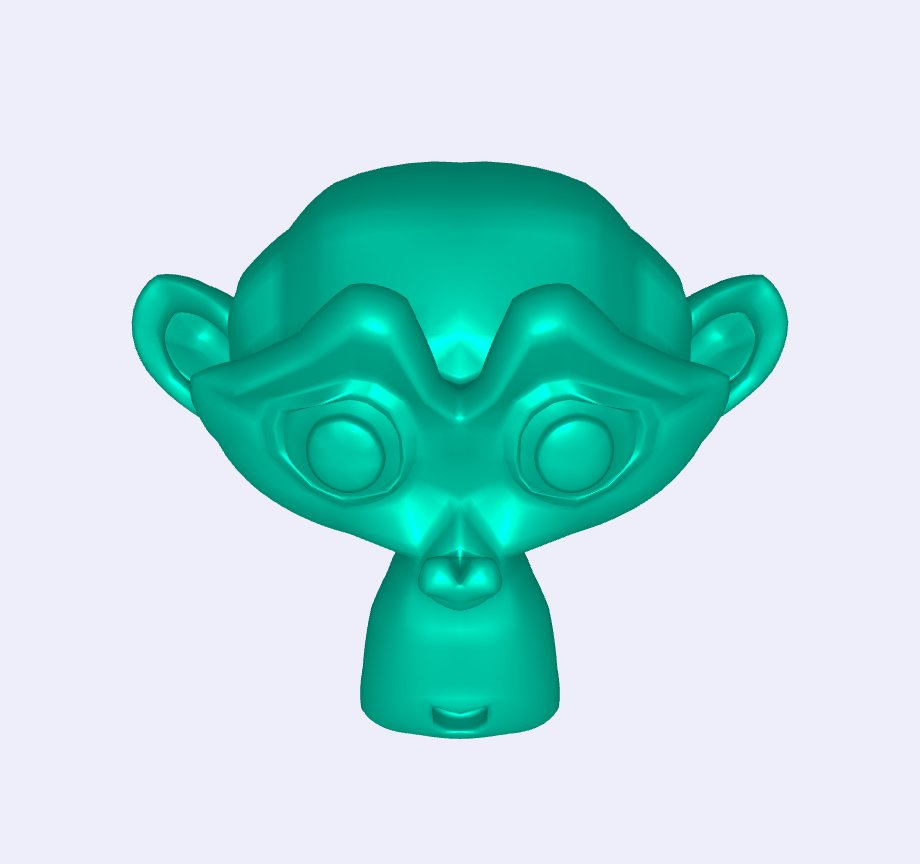
\includegraphics[scale=0.3]{monkey_plastic.png}}
\caption{Model osjenčan difuznom rasvjetom}
\end{center}
\end{figure}

\subsection{Cel-shading princip}

\begin{figure}[H]
\label{fig:monkey-toonshaded}
\begin{center}
\fbox{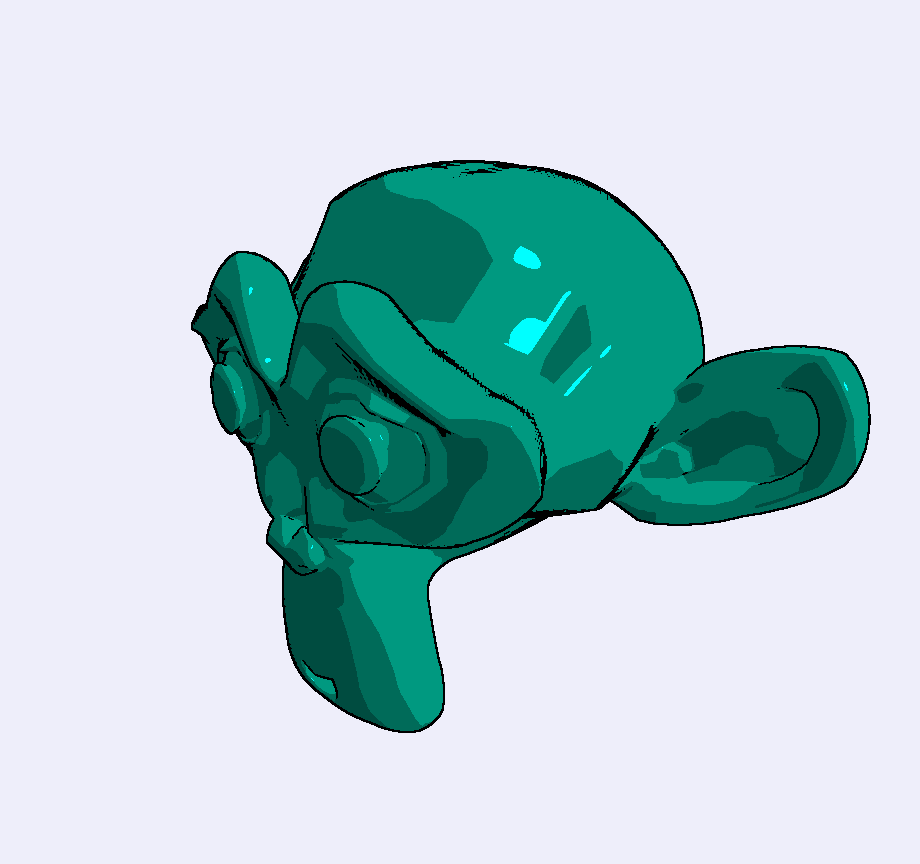
\includegraphics[scale=0.3]{monkey_toonshaded.png}}
\caption{Model osjenčan toon shaderom}
\end{center}
\end{figure}

Što je to uopće i kako se postiže. Koji koraci(slojevi) su potrebni

\subsection{Iscrtavanje obrisa i rubova}

\begin{figure}[H]
\label{fig:monkey-depth}
\begin{center}
\fbox{
\includegraphics[scale=0.3]{monkey_depth.png}}
\caption{Model s iscrtanom \emph{dubinom} pixel-a}
\end{center}
\end{figure}


\begin{figure}[H]
\label{fig:monkey-edges}
\begin{center}
\fbox{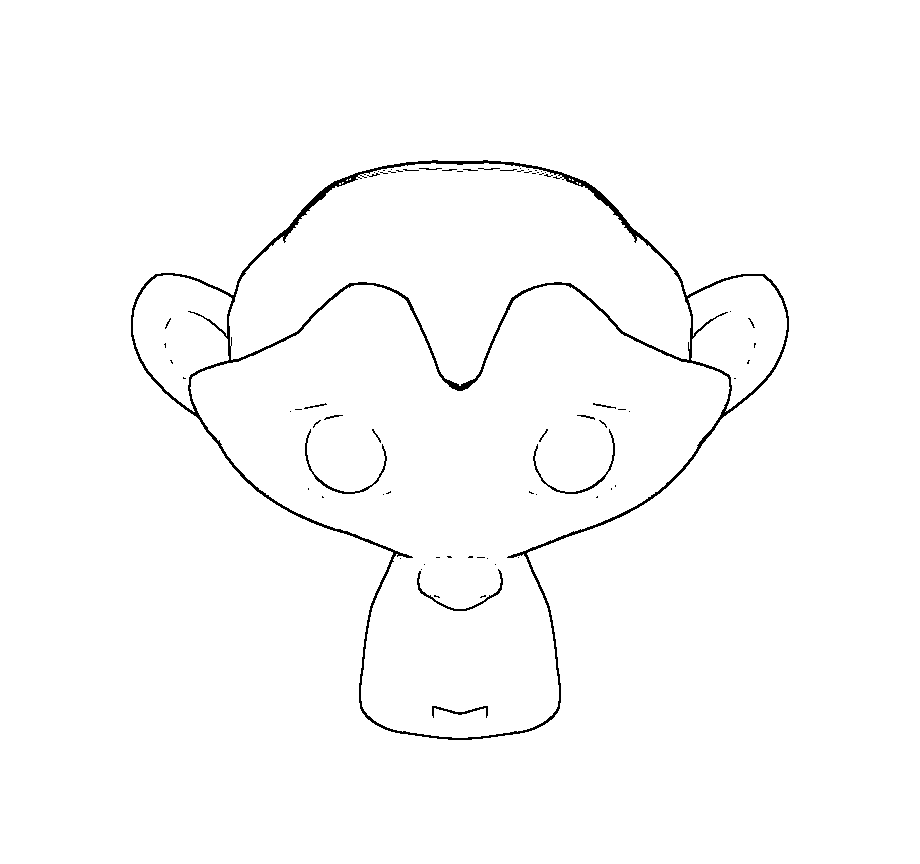
\includegraphics[scale=0.3]{monkey_edges.png}}
\caption{Model s iscrtanim obrisima}
\end{center}
\end{figure}

\subsection{Sjenčanje}

\begin{figure}[H]
\label{fig:monkey-toon}
\begin{center}
\fbox{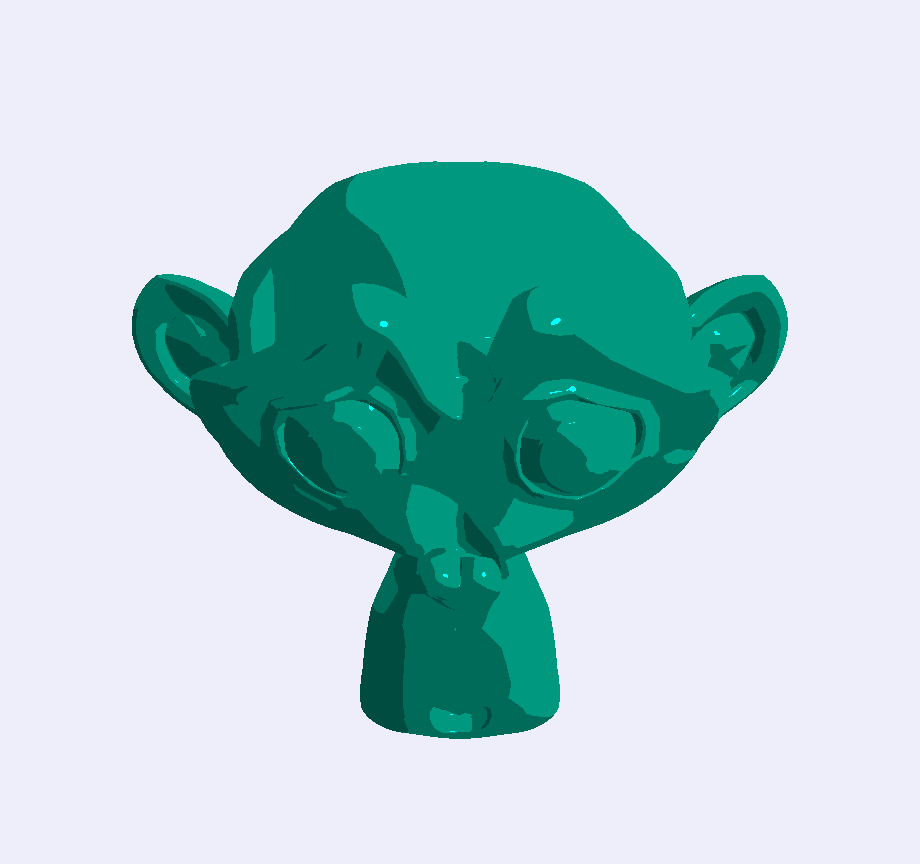
\includegraphics[scale=0.3]{monkey_toon.png}}
\caption{Osjenčani model}
\end{center}
\end{figure}

\subsection{Spajanje slojeva}

\begin{figure}[H]
\label{fig:monkey-final}
\begin{center}
\fbox{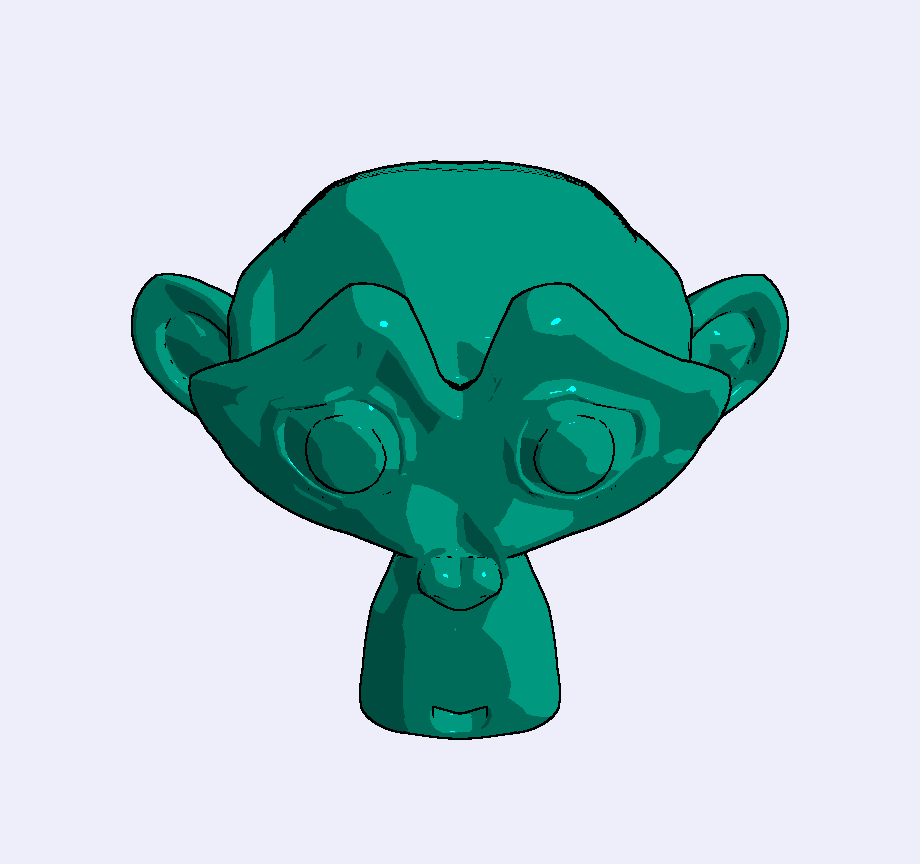
\includegraphics[scale=0.3]{monkey_final.png}}
\caption{Rezultat dobiven spajanjem slojeva}
\end{center}
\end{figure}

Kako se spajaju u cjelinu i što dobijemo s time. Spomenuti ograničenje WebGL-a ovdje
\section{Implementacija}

Prethodna poglavlja opisivala su metodu \emph{toon shading}-a, te način implementacija koji se svodi na izradu \emph{shader} programa. No sam \emph{shader} program, izvodi se na grafičkoj kartici. U ovom poglavlju opisuje se sučelje koje je izrađeno za potrebe rada, koje krajnjem korisniku omogućava izmjenu modela i \emph{shader} programa. Opisuje se način implemntacija, te interakcija sa grafičkom karticom korištenjem \emph{three.js} biblioteke za rad s WebGL-om.

Aplikacija je izrađena pomoću HTML5 tehnologija i \emph{JavaScrip} programskog jezika. Na taj način, omogućeno je izvršavanje neovisno o platofrmi na većini modernih internet preglednika, te uređajima koji podržavaju HTML5 \emph{canvas} element. Budući da mogućnost izvršavanja aplikacija ovisi o grafičkom procesoru i karakteristikama samoga uređaja, korištena je biblioteka \emph{modernizer}\footnote{https://modernizr.com/} za određivanje sklopovske podrške samoga uređaja na kojemu se aplikacija izvršava.

\subsection{Korištenje \emph{three.js}-a}

Opisati framework i u čemu nam pomaže

\subsection{Učitavanje modela}

Na koji način se učitavaju modeli

\subsection{Korištenje više slojeva}

Multi-pass rendering u THREE.js-u
\section{Zaključak}

U ovom radu je prikazan, objašnjen i programski ostvaren \emph{toon shader} način sjenčanja, kao i popratna aplikacija koja omogućava izvršavanje \emph{shader} korisničkoga programa. U teorijskom dijelu opisane su korištene tehnologije, način rada modernih grafičkih kartica kao i osnove tranformacije objekata u 3D prostoru, kao i način rada \emph{toon-shading} algoritma. Također je opisan način rada i korištenja korisničke aplikacije koja se koristi za pregled rezultata i unos podataka.

Na temelju izrađenoga programskog rješenja prikazan je način korištenja \emph{OpenGL}-a, odnosno \emph{WebGL}-a pomoću \emph{three.js} biblioteke. Za potrebe rada samoga algoritma opisan je način detekcije rubova na računalnoj slici, te difuzni način sjenčanja, kao i njegova pojednsotavljena varijanta. Prikazano je na koji način se implementiraju algoritmi sjenčanje koji zahtjeva rad u više iteracija, te kako se problem međuspremnik rješava korištenjem \emph{OpenGL} teksturama.

Izradom korisničkog sučelja, prikazan je način implementacije koji omogućava izvršavanje aplikacije neovisno o uređaju i operativnom sustavu na kojem se aplikacija izvršava, pri čemu su korištene \emph{HTML 5} tehnologije i \emph{JavaScript} programski jezik

Prilikom izrade aplikacije, uočeno je ograničenje \emph{OpenGL} implementacije, koje onemogućava implementaciju algoritma u jednoj iteraciji. Iako je stapanje određenih koraka u jednu iteraciju smanjilo kompleksnost algoritma, on i dalje zahtjeva više od jednoga koraka. Kao posljedica ovoga, krajnja aplikacija j tri puta sporija od jednostavnijih \emph{shader}  korisničkih programa.

\begin{thebibliography}{9}

\bibitem{opengl-wiki-hostory}
	https://www.opengl.org/wiki/History\_of\_OpenGL, posjećeno u lipnju 2016.g.

\bibitem{opengl-wiki-pipeline}
	https://www.opengl.org/wiki/Rendering\_Pipeline\_Overview, posjećeno u lipnju 2016.g.
	
\bibitem{opengl-es-mvp}
	Dan Ginsburg, Budirijanto Purnomo: OpenGL ES 3.0 Programming Gide, Second Edition, 2014.g.

\bibitem{threejs-json}
	https://github.com/mrdoob/three.js/wiki/JSON-Model-format-3, posjećeno u lipnju 2016.g.

\bibitem{opencv-canny}
	http://docs.opencv.org/2.4/doc/tutorials/imgproc/imgtrans/canny\_detector/canny\_detector.html, posjećeno u lipnju 2016.g.

\bibitem{threejs-github}
	https://github.com/mrdoob/three.js, posjećeno u lipnju 2016.g.

\end{thebibliography}

\section*{Sažetak}

U ovom diplomskom radu je opisan i programski ostvaren algoritam za \emph{toon shading} način sjenčanja 3D modela, kao i popratna korisnička aplikacija koja krajnjem korisniku omogućava izvršavanje \emph{shader} korisničkoga programa na grafičkoj kartici računala. Prikazan je način rada algoritma, kao i način implementacije korištenjem \emph{JavaScript} programskog jezika i \emph{JavaScript} biblioteke. Neke od prednosti ovakvoga pristupa su mogućnost izvršavanja programskoga koda neovisno o platformi i operativnom sustavu, te jednostavnost implementacije. Uočeni nedostaci algoritma su nemogućnost implmentacije u jednoj iteraciji, što u konačni negativno utječe na performanse aplikacije.

\textbf{Ključne riječi} sjenčanje 3D modela, detekcija rubova, OpenGL, WebGl, Toon shader, sjenčanje u više iteracija

\section*{Abstract}

This thesis describes and implements algorithm for \emph{toon shading} of 3D models, as well as a supporting application which enables end user to execute shader program on computers graphic card.  It also demonstrates how underlying algorithm works, as well as implementation of it using \emph{JavaScript} programming language and \emph{JavaScript} library. Some of the advantages of this approach are cross platform and operating system independent execution of application, as well as ease of implementation. Observed disadvantage of this approach is forced use of multipass rendering, which has negative impact on applications performance.


\textbf{Keywords} shading of 3D models, edge detection, OpenGL, WebGL, Toon shading, multipass rendering
\section*{Životopis}

Stjepan Udovičić rođen je 15. svibnja 1988 u Osijeku u Republici Hrvatskoj. 2003. godine upisuje se u III. gimnaziju u Osijeku, koju je završio 2007. godine. Tijekom tog razdoblja sudjelovao je natjecanjima iz kemije i informatike. 2007.godine upisuje se na sveučilišni preddiplomski studij računarstva na Elektrotehničkom fakultetu u Osijeku, koji dovršava 2010.g, te nastavlja obrazovanje na sveučilišnom diplomskom studiju procesnog računarstva. Od 2014. godine, zaposlen je u tvrtci Inchoo d.o.o. kao web developer te se bavi izradom web trgovina na Magento platformi.

\section*{Prilozi}

Prilozi na CD-u:

\begin{itemize}
\item \textbf{Prilog 1.} Programski kod aplikacije
\item \textbf{Prilog 2.} udovicic\_stjepan\_diplomski.pdf
\end{itemize}

Nakon  objave rada, programski kod aplikacije te rad u izvornom i PDF formatu moguće je preuzeti na lokaciji:

\begin{itemize}
\item https://github.com/udovicic/WebGL-Test-suite
\end{itemize}
\end{document}
